\documentclass[slidetop,11pt]{beamer}
%
% Ces deux lignes {\`a} d{\'e}commenter pour sortir 
% le texte en classe article
% \documentclass[class=article,11pt,a4paper]{beamer}
% \usepackage{beamerbasearticle}

% Packages pour les fran\c{c}ais
%
\usepackage[T1]{fontenc} 
\usepackage[latin1]{inputenc}
\usepackage[frenchb]{babel}
% pour un pdf lisible {\`a} l'{\'e}cran si on ne dispose pas 
% des fontes cmsuper ou lmodern
%\usepackage{lmodern}
\usepackage{aeguill}

% Pour afficher le pdf en plein ecran
% (comment{\'e} pour imprimer les transparents et pour les tests)
%\hypersetup{pdfpagemode=FullScreen}

% ------------------------------------------------
%-----------   styles pour beamer   --------------
% ------------------------------------------------
%
% ------------- Choix des couleurs ---------------

%% %% %% %% %% COULEURS PERSOS
\definecolor{verylightblack}{rgb}{0.25,0.25,0.25}
\definecolor{lightblack}{rgb}{0.1,0.1,0.1}
\definecolor{black}{rgb}{0,0,0}


\definecolor{verylightgrey}{rgb}{0.8,0.8,0.8}
\definecolor{lightgrey}{rgb}{0.6,0.6,0.6}
\definecolor{grey}{rgb}{0.4,0.4,0.4}

\definecolor{verylightgray}{gray}{0.80}
\definecolor{lightgray}{gray}{0.6}
\definecolor{gray}{gray}{0.4}

\definecolor{verylightblue}{rgb}{0.9,0.9,1.0}
\definecolor{lightblue}{rgb}{0.75,0.75,1.0}
\definecolor{blue}{rgb}{0.5,0.5,1.0}
\definecolor{darkblue}{rgb}{0.0,0.0,0.5}

\definecolor{verylightred}{rgb}{1.0,0.9,0.9}
\definecolor{lightred}{rgb}{1.0,0.75,0.75}
\definecolor{red}{rgb}{1.0,0.5,0.5}

\definecolor{verylightgreen}{rgb}{0.9,1.0,0.9}
\definecolor{lightgreen}{rgb}{0.75,1.0,0.75}
\definecolor{green}{rgb}{0.5,1.0,0.5}


\definecolor{verylightcolorGREY}{gray}{0.80}
\definecolor{lightcolorGREY}{gray}{0.60}

\definecolor{verylightcolorRED}{rgb}{1.0,0.9,0.9}
\definecolor{lightcolorRED}{rgb}{1.0,0.75,0.75}

\definecolor{verylightcolorUN}{rgb}{1.0,0.75,1.0}
\definecolor{lightcolorUN}{rgb}{1.0,0.50,1.0}

\definecolor{verylightcolorDE}{rgb}{0.75,1.0,1.0}
\definecolor{lightcolorDE}{rgb}{0.50,1.0,1.0}

\definecolor{verylightcolorTR}{rgb}{1.0,1.0,0.75}
\definecolor{lightcolorTR}{rgb}{1.0,1.0,0.50}


% Red{\'e}finit la couleur de fond pour imprimer sur transparents
%\xdefinecolor{fondtexte}{rgb}{1,1,1}     % blanc

% commande differente pour les couleurs nomm{\'e}es - de base
%\colorlet{coultexte}{black} 

% -------------- Fioritures de style -------------
% Fait afficher l'ensemble du frame 
% en peu lisible (gris clair) d{\`e}s l'ouverture
\beamertemplatetransparentcovered

% Supprimer les icones de navigation (pour les transparents)
%\setbeamertemplate{navigation symbols}{}

% Mettre les icones de navigation en mode vertical (pour projection)
%\setbeamertemplate{navigation symbols}[vertical]

% ------------ Choix des th{\`e}mes ------------------
\usecolortheme{default} % gabywald
% \usecolortheme{orchid}

\setbeamercolor{title}{fg=black, bg=red!40}
\setbeamercolor{block title}{fg=black, bg=red!40}
\setbeamercolor{structure}{fg=black, bg=red!40}
\setbeamercolor{block title}{fg=black, bg=lightred!40}
\setbeamercolor{substructure}{fg=black, bg=verylightred!40}

\setbeamercolor{block title GREY}{fg=black, bg=lightcolorGREY!40}
\setbeamercolor{substructureGREY}{fg=black, bg=verylightcolorGREY!40}

\setbeamercolor{block title RED}{fg=black, bg=lightcolorRED!40}
\setbeamercolor{substructureRED}{fg=black, bg=verylightcolorRED!40}

\setbeamercolor{block title UN}{fg=black, bg=lightcolorUN!40}
\setbeamercolor{substructureUN}{fg=black, bg=verylightcolorUN!40}

\setbeamercolor{block title DE}{fg=black, bg=lightcolorDE!40}
\setbeamercolor{substructureDE}{fg=black, bg=verylightcolorDE!40}

\setbeamercolor{block title TR}{fg=black, bg=lightcolorTR!40}
\setbeamercolor{substructureTR}{fg=black, bg=verylightcolorTR!40}

% \setbeamercolor{block title}{fg=black, bg=lightblue!40}
% \setbeamercolor{block body}{...}
% \setbeamercolor{block title example}{...}
% \setbeamercolor{block body example}{...}
% \setbeamercolor{block title alerted}{...}
% \setbeamercolor{block body alerted}{...}

% \useoutertheme[left]{sidebar}
% \setbeamersize{sidebar left width=3.0cm \tableofcontents[hideothersubsections] }
% \setbeamercolor{sidebar left}{fg=green,bg=lightgreen}
% \setbeamercolor{title in sidebar}{parent=title}

\setbeamercolor*{sidebar}{fg=lightblack,bg=lightblue!75!white}

\setbeamercolor*{palette sidebar primary}{fg=darkblue!50!lightgrey}
\setbeamercolor*{palette sidebar secondary}{fg=black} % darkblue!10!black
\setbeamercolor*{palette sidebar tertiary}{fg=darkblue!50!lightgrey}
\setbeamercolor*{palette sidebar quaternary}{fg=black} % darkblue!10!black

% \setbeamercolor{subsubsection in sidebar}{hideallsubsections}
% \setbeamercolor{subsubsection in sidebar shaded}{hideallsubsections}


%------------ fin style beamer -------------------

% Faire appara{\^i}tre un sommaire avant chaque section
% \AtBeginSection[]{
%   \begin{frame}
%   \frametitle{Plan}
%   \medskip
%   %%% affiche en d{\'e}but de chaque section, les noms de sections et
%   %%% noms de sous-sections de la section en cours.
%   \small \tableofcontents[currentsection, hideothersubsections]
%   \end{frame} 
% }

% ----------- Contenu de la page de titre --------
\title{La Ligue Ludique Pr{\'e}sente : }
\subtitle{Du sc{\'e}nario de Jeu de R{\^o}le (JdR) au Roman : \newline {\'e}l{\'e}ments d'intrigues} %% \subtitle{Cr{\'e}er une Intrigue (cas du JdR)}
% \author{Gabriel Chandesris & Nicolas Dagron}
% \institute{LigueLudique}
\institute{
\includegraphics[width=5cm]{img/ligueludique-1.png}}
\date{03 Janvier 2018} %% \date{\today} %% \date{03 Janvier 2018}
%% \logo{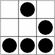
\includegraphics[height=0.5cm]{img/logo_glider.png}}

% ----------- Nom des diff{\'e}rentes parties --------

%% Mis au fur et {\`a} mesure...

\def\moreInFrameTitleLeftt{
\includegraphics[height=0.5cm]{img/ligueludique-0.png}~~~~~}
\def\moreInFrameTitleRight{~~~~~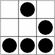
\includegraphics[height=0.5cm]{img/logo_glider.png}}

% ------------------------------------------------
% -------------   D{\'e}but document   ---------------
% ------------------------------------------------
\begin{document}
%--------- {\'e}criture de la page de titre ----------
% avec la commande frame simplifi{\'e}e
\frame[plain]{\titlepage}
%

%------------------ Sommaire ---------------

\begin{frame}
	\frametitle{\moreInFrameTitleLeftt Sommaire \moreInFrameTitleRight}
	\small \tableofcontents[hideallsubsections]
\end{frame} 


%***************************************
%******     I Pr{\'e}sentation  *******
%***************************************
\def\sectionPartI{Pr{\'e}sentation de la Ligue Ludique}
\section{\sectionPartI}
\begin{frame}
	\frametitle{\moreInFrameTitleLeftt \sectionPartI}
	\tableofcontents[sections=1,currentsection,subsectionstyle=show/shaded/hide] %% sectionstyle=hide/hide,
\end{frame} 

\def\sectionPartIa{La Ligue Ludique}
\subsection{\sectionPartIa}
\begin{frame}
	\frametitle{\moreInFrameTitleLeftt \sectionPartIa}
	\tableofcontents[sections=1,currentsection,subsectionstyle=show/shaded/hide]
\end{frame}

\def\sectionPartIaUN{Ligue Ludique... Jeux de R{\^o}le ! }
\subsubsection{\sectionPartIaUN}
\begin{frame}
	\frametitle{\moreInFrameTitleLeftt \sectionPartIaUN}
	\begin{columns}[T]
		\begin{column}[T]{3.5cm}
			
\includegraphics[height=3.4cm]{img/ligueludique-1.png} %% {img/omnesDOCETubique.png}
		\end{column}
		\begin{column}[T]{7cm}
			 \begin{beamerboxesrounded}	[lower=substructureRED, %
							 upper=block title RED,%
							 shadow=true]%
				   {\sectionPartIaUN}
				\begin{itemize}
					\item Association loi 1901, fond{\'e}e en 2008, 
					\item Promotion du JdR (Jeu de R{\^o}le) sur Paris et proche banlieue, 
					\item Parties ouvertes au format court en semaine, 
					\item Partenariats (boutiques, caf{\'e}s...), 
					\item Conventions, salons, {\'e}v{\`e}nements... 
					\item $\Rightarrow$ \underline{\textbf{http://www.ligue-ludique.fr}} $\Leftarrow$
					\item ...
				\end{itemize}
			\end{beamerboxesrounded}
		\end{column}
	\end{columns}
\end{frame}

% ***************************************
% ******     II Th{\'e}matique  	*******
% ***************************************

\def\sectionPartII{Cr{\'e}er une intrigue de JdR}
\section{\sectionPartII}
\begin{frame}
	\frametitle{\moreInFrameTitleLeftt \sectionPartII}
	\tableofcontents[sections=2,currentsection,subsectionstyle=show/shaded/hide] %% sectionstyle=hide/hide,
\end{frame} 

\def\sectionPartIIa{Quelques canevas de base}
\subsection{\sectionPartIIa}
\begin{frame}
	\frametitle{\moreInFrameTitleLeftt \sectionPartIIa }
	\tableofcontents[sections=2,currentsection,subsectionstyle=show/shaded/hide]
\end{frame} 

\def\sectionPartIIaII{Canevas de base}
\subsubsection{\sectionPartIIaII}
\begin{frame}
	\frametitle{\moreInFrameTitleLeftt \sectionPartIIaII  (1)}
	\begin{itemize}
		\item Petites histoires et grandes histoires ; 
		\item Un sc{\'e}nario de JdR (Jeu de R{\^o}le) : un MJ et des Joueurs... 
		\item Personnages Joueurs (PJ) et Personnages Non Joueurs (PNJ) !
		\item Points de vue diff{\'e}rents, narration diff{\'e}rente ;-)
		\item Diff{\'e}rentes histoires qui se croisent, une intrigue commune. 
		\item Intrigues de fond et "d{\'e}cors"...
	\end{itemize}
\end{frame} 

%% img/scenariosHistoires/LecritureDuScenarioSylvainDelzantJeanMarcLaineEditionsEyrolles9782212251128.png
% \begin{frame}
	% \frametitle{\moreInFrameTitleLeftt \sectionPartIIaII  (2)}
	% \begin{columns}[T]
		% \begin{column}[T]{5.05cm}
			% \begin{itemize}
				% \item Rom{\'e}o et Juliette : un gar\c{c}on rencontre une fille, ou inversement, et la perd, la retrouve, etc. 
				% \item Orph{\'e}e aux enfers : la qu{\^e}te de quelqu'un ou quelque chose qui a disparu. 
				% \item Cendrillon : le Bien triomphe malgr{\'e} les difficult{\'e}s rencontr{\'e}es au cours du r{\'e}cit. 
				% \item Faust : la Faute qui doit {\^e}tre expi{\'e}e, le Destin qui frappe t{\^o}t ou tard. 
				% \item Circ{\'e}e : la femme fatale, l'araign{\'e}e et la mouche... 
				% \item Achille : le d{\'e}faut cach{\'e} qui met en danger le h{\'e}ros. 
				% \item Tristan et Yseult : le triangle classique. 
				% \item Le Juif Errant : le voyageur qui n'atteindra jamais son but. 
			% \end{itemize}
			
			% \emph{L'{\'e}criture du sc{\'e}nario}, par Sylvain Delzant, Jean-Marc Lain{\'e}, {\'E}ditions Eyrolles ISBN 9782212251128~\\
			% $\rightarrow$ p14 (reprise int{\'e}grale BD "\emph{La guerre {\'e}ternelle}, suivi de \emph{La libert{\'e} {\'e}ternelle}..." (Joe Haldeman et Marvano)
		% \end{column}
		% \begin{column}[T]{5.05cm}
			% 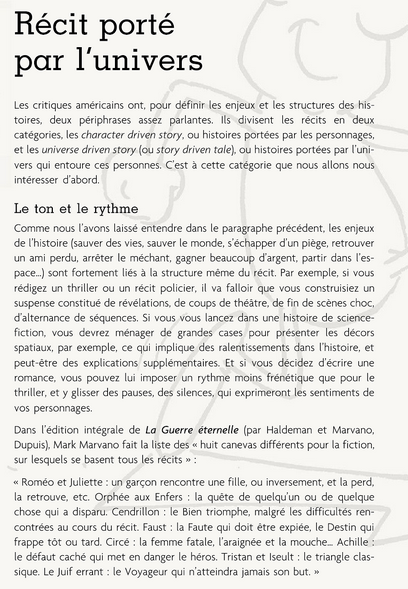
\includegraphics[width=5.00cm]{img/scenariosHistoires/LecritureDuScenarioSylvainDelzantJeanMarcLaineEditionsEyrolles9782212251128.png}~\\
			% \texttt{\footnotesize huit (8) canevas basiques} \newline <<\emph{Genres et personnages non contractuels}>>
		% \end{column}
	% \end{columns}
% \end{frame}

\begin{frame}
	\frametitle{\moreInFrameTitleLeftt \sectionPartIIaII  (2)}
	\emph{"Genres et personnages non contractuels"}
	\begin{itemize}
		\footnotesize
		\item Rom{\'e}o et Juliette : un gar\c{c}on rencontre une fille, ou inversement, et la perd, la retrouve, etc. 
		\item Orph{\'e}e aux enfers : la qu{\^e}te de quelqu'un ou quelque chose qui a disparu. 
		\item Cendrillon : le Bien triomphe malgr{\'e} les difficult{\'e}s rencontr{\'e}es au cours du r{\'e}cit. 
		\item Faust : la Faute qui doit {\^e}tre expi{\'e}e, le Destin qui frappe t{\^o}t ou tard. 
		\item Circ{\'e}e : la femme fatale, l'araign{\'e}e et la mouche... 
		\item Achille : le d{\'e}faut cach{\'e} qui met en danger le h{\'e}ros. 
		\item Tristan et Yseult : le triangle classique. 
		\item Le Juif Errant : le voyageur qui n'atteindra jamais son but. 
	\end{itemize}~\\
	
	\emph{L'{\'e}criture du sc{\'e}nario}, par Sylvain Delzant, Jean-Marc Lain{\'e}, {\'E}ditions Eyrolles ISBN 9782212251128~\\
	$\rightarrow$ p14 (reprise int{\'e}grale BD "\emph{La guerre {\'e}ternelle}, suivi de \emph{La libert{\'e} {\'e}ternelle}..." (Joe Haldeman et Marvano) )
\end{frame}

%% \begin{frame}
%% 	\frametitle{\moreInFrameTitleLeftt \sectionPartIIaII  (3)}
%% 	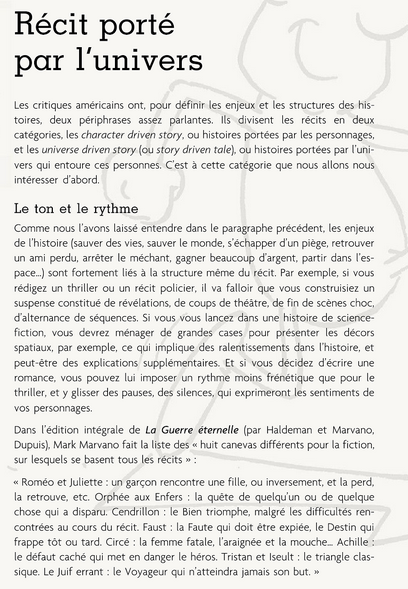
\includegraphics[width=5.00cm]{img/scenariosHistoires/LecritureDuScenarioSylvainDelzantJeanMarcLaineEditionsEyrolles9782212251128.png}~\\
%% 	\texttt{\footnotesize huit (8) canevas basiques} \newline "\emph{Genres et personnages non contractuels}"
%% \end{frame}

\def\sectionPartIIb{Grande Liste des Intrigues de JdR}
\subsection{\sectionPartIIb}
\begin{frame}
	\frametitle{\moreInFrameTitleLeftt \sectionPartIIb }
	\tableofcontents[sections=2,currentsection,subsectionstyle=show/shaded/hide]
\end{frame} 


\def\sectionPartIIbI{Les parties d'une histoire}
\subsubsection{\sectionPartIIbI}
\begin{frame}
	\frametitle{\moreInFrameTitleLeftt \sectionPartIIbI}
	\begin{enumerate}
		\item \textbf{L'intrigue. }Forme premi{\`e}re de l'histoire, incluant des incidents majeurs et des rencontres. D{\'e}fini par le MJ. Les joueurs peuvent cr{\'e}er tout ou partie des sous-intrigues.
		\item \textbf{Conflit et strat{\'e}gie. }Comment les PJ vont-ils r{\'e}soudre leurs probl{\`e}mes ?
		\item \textbf{Personnages. }Le MJ apporte beaucoup d'interpr{\'e}tation, mais les joueurs fournissent l'essentiel du roleplay.
		\item \textbf{Dialogue. }Joueurs et MJ se r{\'e}partissent cette t{\^a}che, qui rel{\`e}ve surtout des joueurs.
		\item \textbf{Univers et th{\`e}me. }La t{\^a}che du MJ.
	\end{enumerate}
\end{frame} 


\def\sectionPartIIbII{36 Intrigues en JdR}
\subsubsection{\sectionPartIIbII  -- Sources}
\begin{frame}
	\frametitle{\moreInFrameTitleLeftt \sectionPartIIbII  -- Sources}
	\begin{itemize}
		\item \emph{La Grande Liste des Intrigues de Jeu de R{\^o}le} \newline
			par S. John Ross, traduction Lo{\"i}c Prot
		\item 36 Intrigues et leurs variantes...
		\item \texttt{http://fudge.ouvaton.org/GrandeListe.html}
		\item cf. \emph{Les 36 sc{\'e}narios} (Loren J. Miller, 1994-1997) \texttt{http://ptgptb.fr/les-36-scenarios}
		\item cf. \emph{Les Trente-Six Situations Dramatiques} (Georges Polti, 1924) ; LE grand classique...
		\item Sur Wikipedia : \texttt{https://fr.wikipedia.org/wiki/36\_situations\_dramatiques}
	\end{itemize}
\end{frame} 

\subsubsection{\sectionPartIIbII  -- (1-6)}
\begin{frame}
	\frametitle{\moreInFrameTitleLeftt \sectionPartIIbII  -- (1-6)}
	\begin{enumerate}
		\item[1] Amn{\'e}sie
		\item[2] Base Cach{\'e}e
		\item[3] Capturer le Drapeau
		\item[4] Chantage
		\item[5] Chasse {\`a} l'Homme
		\item[6] Concours
	\end{enumerate}
\end{frame} 

\subsubsection{\sectionPartIIbII  -- (7-12)}
\begin{frame}
	\frametitle{\moreInFrameTitleLeftt \sectionPartIIbII  -- (7-12)}
	\begin{enumerate}
		\item[7] Course au Tr{\'e}sor
		\item[8] D{\'e}fense (Ils ne passeront pas)
		\item[9] D{\'e}placement (On est o{\`u}, l{\`a} ?)
		\item[10] D{\'e}tournement
		\item[11] Diplomatie (Les Bonnes Mani{\`e}res)
		\item[12] Effraction
	\end{enumerate}
\end{frame} 

\subsubsection{\sectionPartIIbII  -- (13-18)}
\begin{frame}
	\frametitle{\moreInFrameTitleLeftt \sectionPartIIbII  -- (13-18)}
	\begin{enumerate}
		\item[13] Enqu{\^e}te ({\'E}l{\'e}mentaire, mon cher Watson)
		\item[14] Escorte
		\item[15] {\'E}trange (Comme c'est bizarre...)
		\item[16] Exploration
		\item[17] Fauteurs de Troubles
		\item[18] Gestion (Au travail !)
	\end{enumerate}
\end{frame} 

\subsubsection{\sectionPartIIbII -- (19-24)}
\begin{frame}
	\frametitle{\moreInFrameTitleLeftt \sectionPartIIbII  -- (19-24)}
	\begin{enumerate}
		\item[19] Grain de Sable
		\item[20] Harc{\`e}lement (Qu'est-ce qui se passe ?)
		\item[21] Nettoyer la Zone
		\item[22] Portail (La Boite de Pandore)
		\item[23] Pourchasser (Rattrapez-les !)
		\item[24] Prison
	\end{enumerate}
\end{frame} 

\subsubsection{\sectionPartIIbII  -- (25-30)}
\begin{frame}
	\frametitle{\moreInFrameTitleLeftt \sectionPartIIbII  -- (25-30)}
	\begin{enumerate}
		\item[25] Qu{\^e}te
		\item[26] Refuge (Un Abri dans la Temp{\^e}te)
		\item[27] Ruines R{\'e}centes
		\item[28] Safari
		\item[29] Secours (Ils sont en Chemin)
		\item[30] Surveillance (Ne Pas Toucher)
	\end{enumerate}
\end{frame} 

\subsubsection{\sectionPartIIbII  -- (31-36)}
\begin{frame}
	\frametitle{\moreInFrameTitleLeftt \sectionPartIIbII  -- (31-36)}
	\begin{enumerate}
		\item[31] Survie (Ne Mangez Pas Les Mauves)
		\item[32] Tr{\'e}sor !
		\item[33] La Zone
		\item[34] De l'autre C{\^o}t{\'e} de la barri{\`e}re
		\item[35] \emph{R{\'e}parations}
		\item[36] \emph{Variantes}
	\end{enumerate}
\end{frame} 

% ***************************************
% ******     III Questions  	*******
% ***************************************

\def\sectionPartIII{Questions}
\section{\sectionPartIII}
\begin{frame}
	\frametitle{\moreInFrameTitleLeftt \sectionPartIII}
	% \tableofcontents[sections=2,currentsection,subsectionstyle=show/shaded/hide] %% sectionstyle=hide/hide,
	Des Questions ?
\end{frame} 

\def\sectionPartIV{Atelier Pratique}
\section{\sectionPartIV}
\begin{frame}
	\frametitle{\moreInFrameTitleLeftt \sectionPartIV}
	% \tableofcontents[sections=2,currentsection,subsectionstyle=show/shaded/hide] %% sectionstyle=hide/hide,
	\begin{itemize}
		\item choisir un fil conducteur pour : 
		\begin{itemize}
			\item un personnage (dans un groupe ?) ; 
			\item un groupe de personnages (2 {\`a} 6) ; 
		\end{itemize}
		\item parmi les intrigues propos{\'e}es (voire plusieures, pour une histoire complexe), 
		\item faire le point de vue des protagonistes (Personnages Joueurs / Personnages Non Joueurs)...
	\end{itemize}
\end{frame} 

\end{document}
